\chapter{Specification}
\section{Purpose}
The prestudy of this thesis gives an insight in the fundamentals of messaging, especially
the purpose of message brokers for big data event streaming. We also compare
the most related broker implementations and provide detailed information about Apache
Kafka. The second part of this work is focusing on the implementation of a message
broker in the functional program language Haskell\todo{ref}. The goal is to get
use of the advantages of the functional paradigm regarding to the resulting
throughput performance. By using the example of Apache Kafka the main purpose
lies on building a server application which implements the main functionality of
Apache Kafka. 

\section{Features}
\begin{table}[h]
\begin{tabular}{lll}
\textbf{Functionality}       & \textbf{Description} & \textbf{Part of Thesis} \\
Server Implementation        &                      & yes                     \\
Wire Protocol Implementation &                      & yes                     \\
API for Haskell Clients      &                      & yes                     \\
Thin Haskell Clients         &                      & yes                     \\
Producing Messages           &                      & yes                     \\
Consuming Messages           &                      & yes                     \\
Log Persistency              &                      & yes                     \\
Error Handling               &                      & yes                     \\
Message Batching             &                      & yes                     \\
Message Compression          &                      & no                      \\
Partitioning                 &                      & partly                  \\
Log Compaction               &                      & no                      \\
Broker Replication           &                      & no                      \\
Broker Recovery              &                      & no                      \\
Consumer Groups              &                      & no                      \\
Zookeeper Integration        &                      & no                     
\end{tabular}
\end{table}

\section{Components}

Basically, the architecture consists of two main components namely the broker and
the client, whereas the client can act as producer, consumer or both. The broker
is a server which only reacts to requests that are sent from clients. Every
request contains an API key which the broker uses to determine which action it
has to do (e.g. persist produced message or consume message). For each valid
request the broker sends back a corresponding response to the client which
either includes the fetched data or an error code. The broker never communicates
with a client without a request.

\begin{figure}[H]
    \centering
     \begin{sequencediagram}
        %\newthread{broker}{Broker}
         \newinst[3]{client}{Client}
         \newinst[3]{broker}{Broker}
        \begin{messcall}
            {client}{(1) Send Request}{broker}{}
        \end{messcall}
        \begin{messcall}
            {broker}{(2) Do Action}{broker}{}
        \end{messcall}
        \begin{messcall}
            {broker}{(3) Send Response}{client}{} 
        \end{messcall}
     \end{sequencediagram}
     \caption{Basic communication between client (producer or consumer) and
     broker}
\end{figure}

\section{Workflow}

The main purpose of this broker implementation can be split in two cases. Case
one covers producing a message and persisting in the brokers log. Case two
allows to consume persisted messages on request. As for clients, depending on
which API to be used, the client can act either as producer or consumer.

\subsection{Producer}

In the case of a producer client, the following workflow highlights the
fundamental steps being passed from sending a request by the client to
persisting the message on the broker.

\begin{figure}[H]
    \centering
    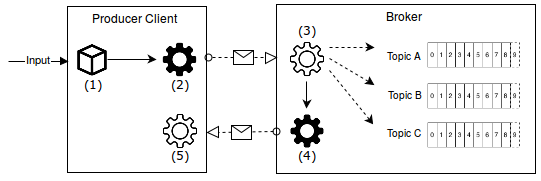
\includegraphics[width=0.8\textwidth]{images/concept_producer.png}
    \caption{Case one: Producer Workflow}
    \label{fig:conept-producer}
\end{figure}

\begin{description}
    \item [(1)] 
        {Packing Produce Request: Getting input data to protocol conform data structure.}
    \item [(2)] 
        {Serializing and send Produdce Request: Encoding data structure to an
            binary  string and transmit over a tcp socket to the broker.}
    \item [(3)] 
        {Parsing and Handling Produce Request: Broker receives the binary string
            and parse it back to the appropriate data structure. The request
            handler of the  broker checks the API Key of the request. If it is a
            produce request, the containg message will be written to the
            appropriate topic log.}
    \item [(4)] 
        {Send Produce Response: A response is packed, serialized and transmitted
            back to the client. The response contains an error code which has
            the value 0 if everything worked well otherwise another value for a
            specific problem. }
    \item [(5)] 
        {Parse Produce Response: Producer client receives a binary string and
            parses it to valid response data structure }
\end{description}

\subsection{Consumer}

The consumer fetches desired messages through requesting it at any time.

\begin{figure}[H]
    \centering
   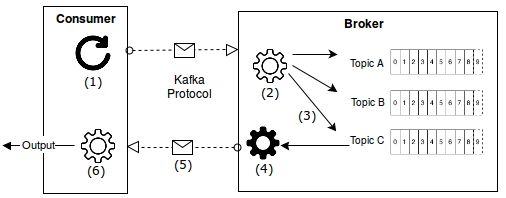
\includegraphics[width=0.7\textwidth]{images/concept_consumer.png}
    \caption{Case two: Consumer Workflow}
    \label{fig:concept-consumer}
\end{figure}

\begin{description}
    \item [(1)] 
        {Continously send fetch request: Consumer client sends fetch
        requests in configurable intervall as binary string to the broker. } 
    \item [(2)] 
        {Parsing and handling fetch request: Broker receives the binary string
            and parse it back to the appropriate data structure. The request
            handler of the broker checks the API Key of the request. If it is a
            fetch request, the broker reads messages of the requested topic and
            packs it to a fetch response. message will be written to the
            appropriate topic log.}
    \item [(3)] 
        {Send fetch response: The fetch request which contains the requested
        messages is send back to the consumer client.}
    \item [(4)] 
        {Parse Response:Consumer client receives a binary string and parses it
        to valid response data structure }
\end{description}

